 %Diese Zeile bitte -nicht- aendern.
 \documentclass[course=erap] {aspdoc}

 %eigene Imports
 \usepackage{amsfonts}
 \usepackage{pgfplots}
 \usepackage{ulem}
 \usepackage{amssymb}
 \pgfplotsset{compat=1.16}
 
 
 %%%%%%%%%%%%%%%%%%%%%%%%%%%%%%%%%
 %% TODO: Ersetzen Sie in den folgenden Zeilen die entsprechenden -Texte-
 %% mit den richtigen Werten.
 \newcommand{\theGroup}{233} % Beispiel: 42
 \newcommand{\theNumber}{A316} % Beispiel: A123
 \author{Ludwig Gröber \and Julian Pins \and Daniel Safyan}
 \date{Sommersemester 2023} % Beispiel: Wintersemester 2019/20
 %%%%%%%%%%%%%%%%%%%%%%%%%%%%%%%%%
 
 % Diese Zeile bitte -nicht- aendern.
 \title{Gruppe \theGroup{} -- Abgabe zu Aufgabe \theNumber}
 
 \begin{document}
     \maketitle
 
 
     \section{Einleitung}
     Die gegebene Aufgabenstellung A316 verlangt die Implementierung der Funktion $\operatorname{f}(x) = arsinh(x)$ im C17 Standard von C.
     Wie die angewandte Methodik und der mathematische Lösungsansatz aussieht, wird im Folgenden beschrieben.
 
     \subsection{Einführung}
     %Allgemeine Einführung und Abwägung bei Optimierungen
     Im Folgenden wird ein Problem aus dem Bereich der optimierung von Programmen behandelt.
     Diese Optimierung kann unter verschiedenen im Folgenden erläuterten Kriterien erfolgen.
     Die Optimierung vom Programmen ist im Allgemeinen immer ein Abwägen zwischen Implementierungsaufwand/Laufzeit in Zyklen/Laufzeit in Zeit/Energieaufwand/Portabilität/Speicherverbrauch und weiteren Anwendungsspezifischen Faktoren. $[das bissl Schmarrn]$
     Diese Abwägungen werden im Folgenden auch bei den Implementierungen getroffen und und es wird versucht ein 'optimales' Ergebnis in verschiedenen Dimensionen zu erzielen, zu messen und zu bewerten.
     Hierbei dient uns der Vergleich als Bewertungskriterium und die bewerteten Dimensionen werden in den weiteren Kapiteln noch genauer spezifiziert.
     Eine Bewertung der Ergebnisse erfolgt am Ende des Kapitels Performanzanalyse.
 
     %Motivation
     Die Gruppe der hyperbolischen Funktionen wird für die Hankel-Transformation~\cite{hankel}, $[bro wasis das]$
     bei der Lösung bestimmter Differenzialgleichungen~\cite{differenzial}, bei der Beschreibung von Katenoiden~\cite{katenoid}
     sowie in den Friedmann-Gleichungen für die zeitliche Entwicklung der Ausdehnung des Universums~\cite{universum1,universum2}~ benötigt. 
     Für diese üblicherweise rechenintensiven Anwendungen ist eine effiziente und genaue Implementierung aller dafür verwendeten Funktionen essenziell um Gesamtergebnisse effizient erzielen zu können.
     Deshalb widmed sich diese Ausarbeitung im folgenden der Implementierung einer hyperbolischen Funktion, dem $arsinh$.
 
     \subsection{Aufgabenstellung analysiert und spezifiziert}
     Die gestellte Aufgabe verlangt die numerische Berechnung der Funktion f(x) = arsinh(x) im C17 Standard von C.
 
 
     %Mathematische Analyse
     Über den komplexen Zahlen $\mathbb{C}$ bildet die Funktion $arsinh$ mehrwertig ab, weshalb die Einschränkung auf die reellen Zahlen $\mathbb{R}$ getroffen wird.
     Die Funktion area sinus hyperbolicus bildet über $\mathbb{R}$ nach $\mathbb{R}$ ab und ist im Bereich $-\infty < x < + \infty$ definiert.
     Der area sinus hyperbolicus kann über den Logarithmus oder über ein Integral definiert werden.
 
     $$ (1) \operatorname{arsinh}(x) = \ln \left(x + \sqrt{x^2 + 1} \right) \, mit \, x \in \mathbb{R}$$
 
     $$ (2) \operatorname{arsinh}(x) = \int_{0}^{1} \frac{x}{\sqrt{x^2 y^2 + 1}} \,\mathrm{dy} \, mit \, x \in \mathbb{R} $$
 
     Im Limit kann er durch die Funktion $ (3) f(x)\to \pm \ln(2|x|)$ angenähert werden.
     Als für die Implementierung relevante mathematische Eigenschaft die Punktsymmetrie zum Ursprung $(0,0)$ bereits hier zu erwähnen. In der folgenden Analyse werden wir daher primär den Wertebereich $x \leq 0$ analysieren. Der negative Fall verhält sich jeweils symmetrisch.
     %Die Familie der hyperbolischen Funktionen sind quadratische rationale Funktionen von der Exponentialfunktion $\exp$,
     %die über die Mitternachtsformel gelöst werden könnten und mit dem natürlichen Logarithmus $\ln$ ausgedrückt werden.
     %Überleitung
     Bei der Abbildung einer stetigen Funktion in ein endliches System müssen zudem Einschränkungen im Wertebereich sowie bei der Genauigkeit getroffen werden.
 
     %Implementierung
     Letzteres wird im eigens dafür vorgesehenen Kapitel Genauigkeit diskutiert, allgemein kann jedoch bereits zum Datentyp $double$ erwähnt werden, dass bei 52 Fragment-bits eine dezimale Genauigkeit von $53*\log10(2) \approx 15,96$ Nachkommastellen die Grenze des Datentyps darstellt.~\cite{StandardforBinaryFloating}
     Erstere Grenze gibt die Aufgabenstellung indirekt durch die doppelte Genauigkeit der Fließkommaarithmetik vor.
     Der Wertebereich der Implementierung ist ebenso durch den Datentypen $double$ beschränkt $\min(double) \approx 2,2250738585072014* 10^{308}$ und $\max(double) \approx 1,7976931348623157 * 10^{308}$
     Die Werte $\pm \infty$ und $\pm NaN$ sind bei $double$ besonders zu beachten.
     Da die Funktion streng monoton steigend ist, definieren wir:
     \[(4) \operatorname{arsinh}(x) =
     \begin{cases}
         arsinh(x)     & \text{ falls } x < \infty \wedge \, x > -\infty \\
         +NaN  & \text{ falls } x = +NaN \\
         -NaN  & \text{ falls } x = -NaN \\
         +\infty     & \text{ falls } x = +\inf \\
         -\infty     & \text{ falls } x = -\inf \\
         +NaN     & \text{ sonst }
 
     \end{cases}\]
     Ein Problem bei $double$ ist zudem die Endianness, die nicht in IEEE 754~\cite{StandardforBinaryFloating-PointArithmetic} spezifiziert ist.
     Es könnte also zu Fehlern zwischen Systemen kommen, die Behandlung dessen übersteigt den Umfang diese Ausarbeitung und wird deshalb aus dem Themenbereich ausgeschlossen.
 
     Neben den sich aus dem Datentyp ergebenden Einschränkungen stellt die Aufgabenstellung ebenso Einschränkungen an arithmetischen Operatoren.
     In den naiven Ausarbeitungen dürfen nur grundlegende Berechnungen, also die vier Grundrechenarten sowie shifts verwendet werden.
     In der weiterführenden Ausarbeitung sind komplexe Berechnungen wie $exp$ oder $log$ sowie SIMD, SSE zugelassen und weitere Optimierungen wie Loop-unrolling, Endrekursion, die Wahl anderer Algorithmen und Datenstrukturen erlaubt und erwünscht.
 
 
     Von den beiden geforderten Vergleichsimplementierungen als Reihenentwicklung und als Tabellen-Lookup ist letztere bereits als eine Form der Optimierung zu verstehen und kann deshalb bereits mit der Reihe, ceteris paribus, verglichen werden.
     Tabellen-Lookup scheint für die gegebene Aufgabe eine gute Optimierung zu sein, da für eine bekannte Menge an Funktionswerten häufige und identische Berechnungen durchgeführt werden.
     Die Wahl der größe eines Tabellen-Lookups ist eine Abwägung zwischen Genauigkeit, Laufzeit und Speicherplatz, dies wird im Folgendem Kapitel Optimierungen weiter erläutert.
 
 
     Gemäß Aufgabenstellung werden drei C-Implementierungen erarbeitet und verglichen.
 
 
     (A) Implementierung als reine Reihendarstellung mit grundlegenden Berechnungen
 
 
     (B) Implementierung als Tabellen-Lookup mit grundlegenden Berechnungen
 
 
     (C) Hauptimplementierung: Eine Implementierung nach freier Wahl mit komplexen Instruktionen
 
     Ebenso wird zum Vergleich eine Implementierung (D) basierend auf der <math.h> Bibliothek verwendet.
 
     Im folgenden werden die Implementierungen mit den respektiven Buchstaben $(A)$ - $(D)$ referenziert, die nummerierten Formeln und Definitionen analog mit den Zahlen $(1)$ - $(4)$. 
     $A$ wird im Folgenden als naive Implementierung und $(D)$ als Benchmark für die Performanz und Genauigkeit verwendet. 
 
 
     Das Rahmenprogramm unterstützt die Funktionen $-V<Zahl>$ für die Wahl der Implementierung, $-B<Zahl>$ für die Wiederholungen des Funktionsaufrufs, $<Floating Point Zahl>$ für den Wert $x$, $-h$ oder $--help$ für die Beschreibung der Optionen des Programms und Verwendungsbeispiele hierfür.
    
 
     Eine Implementierung in Assembly ist nicht gefordert und es wird in dieser Ausarbeitung auch darauf verzichtet, da der Fokus im Folgenden auf Genauigkeit und nicht auf Performanz liegen wird.
     Ebenso wird auf Mikro-Optimierungen verzichtet, da es allgemein schwer ist moderne Compiler in Optimierungsaufgaben zu schlagen und der Code hierdurch schwerer zu lesen, fehleranfälliger und schwerer zu warten wird.
     Dies steht allgemein best-practices im Software-Engineering entgegen.
 
 
     \section{Lösungsansatz}
 
     Sowohl für die Implementierung mit einer Reihendarstellung, als auch für die Lookuptabelle haben wir uns die Punktsymmetrie der $arsinh$-Funktion zunutze gemacht: $arsinh(-x) = -arsinh(x)$. Die Funktionswerte für negative Eingabewerte, werden als $-arsinh(|x|)$ berechnet.
     \subsection{Reihendarstellung}
     Da Reihenentwicklungen in der Regel nur begrenzte Gültigkeitsbereiche haben, verwenden wir verschiedene Reihen für die Intervalle $|x| < 1$ und $|x| > 1$:
       \[ \operatorname{arsinh}(x) =
     \begin{cases}
         \sum_{k = 0}^{\infty} \frac{(-1)^k(2k)!x^{2k + 1}}{(2k + 1)(2^k*k!)^2}     & \text{ falls } |x| < 1 \\
         ln(2x) + \sum_{k = 1}^{\infty} \frac{(-1)^{k - 1}(2k)!x^{2k + 1}}{2k(2^k\cdot k!)^2} \cdot \frac{1}{x^{2k}}  & \text{ falls } |x| >1 \\
         x     & \text{ falls } x \in \{\pm\inf, \pm Nan\}\\
     \end{cases}\]
     Diese Berechnungen sollen im Folgenden näher erläutert werden:
     
     Für $|x| < 1$ wird die Taylor-Reihe des $arsinh(x)$ um den Entwicklungspunkt 0 verwendet:
     \[
         arsinh(x) = \sum_{k = 0}^{\infty} \frac{(2k-1)!!(-x^2)^k}{(2k)!!(2k + 1)}
         = \sum_{k = 0}^{\infty} \frac{(-1)^k(2k)!x^{2k + 1}}{(2k + 1)(2^k*k!)^2}
     \]
     Durch das Auflösen der Doppelfakultäten entsteht eine deutlich leichter implementierbare Formel.
     Da diese Reihe nur gültig ist für $|x| < 1$, werden für Werte außerhalb dieses Wertebereichs die anderen Reihen herangezogen.
     %x>1
 
     Die Berechnung für $|x| > 1$ folgt aus folgender Näherung:
     \[
         arsinh(x) = \ln(x + \sqrt{x^2 + 1}) = \ln(2x) + error(x)
     \]
     Der Fehler dieser Näherung kann durch eine dritte Reihe berechnet werden, was für den Funktionswert für $|x| < 2^{8}$ essentiell ist:
     \[
         error(x) =  \sum_{k = 1}^{\infty} \frac{(-1)^{k - 1}(2k)!x^{2k + 1}}{2k(2^k\cdot k!)^2} \cdot \frac{1}{x^{2k}}
     \]
     Für die Berechnung von $\ln(2x)$ verwenden wir die Taylorreihe des natürlichen Logarithmus um den Entwicklungspunkt 1. Es gilt zu beachten, dass diese Reihe nur im Wertebereich $[0, 2]$ Gültigkeit hat.
     \[
         \ln(x) = \sum_{k = 1}^{\infty} \frac{(-1)^{k + 1}}{k}(x - 1)^k
     \]
     Aufgrund der begrenzten Gültigkeit der Reihe müssen wir uns das $double$ Datenformat zunutze machen, um die Berechnung zu optimieren. Durch eine Bitmaske lassen sich effizient Exponent und Mantisse von $x$ ermitteln. Mit Exponent und Mantisse lässt sich nun folgende Umformung treffen:
     \begin{gather*}
         x = M\cdot2^E \,\,\, mit \,\,\, M = implizierte Mantisse \,\,\, E = implizierter Exponent\\
         arsinh(x) \approx \ln(2x) = \ln(2) + \ln(x) = \ln(2) + \ln(M\cdot2^E) = \ln(2) + E\cdot\ln(2) + \ln(M)\\ = (E+1)\cdot\ln(2) + \ln(M)
     \end{gather*}
     Da $M\in[1, 2[$ liegt, kann nun die Taylorreihe für die Berechnung von $\ln(M)$ verwendet werden. Es gilt jedoch zu beachten, dass die Taylorreihe berits für wenige Reihenglieder exaktere Ergebnisse liefert, je näher der zu berechnende Wert an Eins liegt. Um weniger Reihenglieder der Taylorreihe für ein exaktes Ergebnis zu benötigen, haben wir uns daher dafür entschieden, alle Werte der Mantisse, die über $1.\overline{3}$ liegen, nochmal zu halbieren und stattdessen den Exponenten um 1 zu erhöhen, damit der Eingabewert für die Taylorreihe möglichst nahe an 1 liegt. Es gilt damit $M\in[0.\overline{6}, 1.\overline{3}]$. 
     $\\$
     Die Koeffizienten der einzelnen Reihenglieder zu berechnen ist extrem Laufzeitaufwendig, da insbesondere die Berechnung der Fakultät viel Zeit kostet. Daher haben wir beschlossen, die Berechnung zu optimieren, indem die Koeffizienten aller drei Reihen bereits vor Runtime berechnet werden. Für die Berechnung eines Reihengliedes muss nun nur noch der entsprechende Koeffizient auf die jeweilige Potenz von $x$ multipliziert werden. Hierbei wird die nächste Potenz von x jeweils aus der Potenz im vorherigen Reihenglied berechnet, um unnötigen Overhead durch erneute Potenzierung zu vermeiden. 
     Die Anzahl an benutzten Reihenglieder, entsteht aus einer Abwägung zwischen Performanz und Genauigkeit welche in folgenden Kapiteln erläutert wird.
     
     \subsection{Tabellen-Lookup}
     Unsere Implementierung des Tabellen-Lookups besteht funktional aus 2 Teilen: Das Mapping vom Inputwert auf
     die zugehörigen Werte in der Tabelle und das Interpolieren zwischen diesen.
     
     %Mapping
     Das Mapping ist eine effiziente, simple Hashfunktion, die die 19 höchstwertigsten Bit (ohne das Signbit) des Double-Inputwerts als Index benutzt. Daran kann man auch sehen, dass
     unsere Tabelle logarithmisch aufgebaut ist $\rightarrow$ Jeder Exponent im Wertebereich hat dieselbe Anzahl an Werten gespeichert. 
     Wir haben uns für eine logarithmische Tabelle wegen dem Aufbau von $doubles$ entschieden. Erstens wird dadurch die Implementatierung
     dieser effizienten Hashfunktion ermöglicht und zweitens ist so in jedem Intervall die Dichte der Einträge im Verhältnis 
     zur Dichte der $double$-Werte fast konstant und führt somit zu einer minimalen Gesamtabweichung(Näheres im Genauigkeitskapitel).
 
     %Interpolation
     Nachdem nun die Hashfunktion einen Index $i=hash(x)$ liefert, gilt: $table[i] \leq arsinh(x) \leq table[i+1]$
     Nun interpolieren wir in diesem Abschnitt linear mit $y_j = table[j]$:
     \[
         arsinh(x) \approx \frac{y_{i+1}-y_i}{\Delta x_{table}}\cdot (x-y_i) + y_i
     \]
     Da $\Delta x_{table}$ jedoch von $i$ abhängt, muss dieses erst bestimmt werden. Dies passiert bei uns 
     effizient, mithilfe der Mantissenbits.
     
     Diese Implementierung verbraucht sehr viel Speicher, ist jedoch sehr schnell. Aber die Approximation, die wir hier vornehmen, ist, dass in dem kurzen Intervall in dem wir interpolieren ändert sich die Steigung nicht. Würden wir also den Speicherverbrauch reduzieren indem wir eine kleinere Tabelle nutzen, würden wir die Genauigkeit senken, da die Intervalle größer würden und die Gesamtkrümmung in den einzelnen Intervallen stiege. Hier gibt also keinen Tradeoff zwischen Genauigkeit und Performanz, sondern Genauigkeit und Speichererffizienz, auf welchen in darauffolgenden Kapiteln näher eingegangen wird.
     \subsubsection{Abwägung Genauigkeit und Performanz}
     \subsubsection{Problematik der "reinen" Reihenentwicklung}
     
 
 
     
     % Theoretischer Teil
     %In diesem Absatz rechtfertigen wir die beiden Ansätze der Reihenentwicklung und des Tabellen-Lookups mathematisch.
     %Sowohl die Polynominterpolation als auch die intervallweise lineare Interpolation sind
     % >>Leiten Sie mathematisch zwei Möglichkeiten her, die Funktion zu berechnen.
     % Verwenden Sie dazu sowohl eine reine Reihendarstellung als auch eine Methodik, die einen Tabellen-Lookup benutzt.
     % Ideen: Reihenentwicklung nicht zur Runtime, sondern zur Compiletime berechnen.
     % Runge Effekt: zwischen Integralgrenzen gut angenähert, wenn mit Polynom genähert wird. -> Deshalb funktioniert die Reihenentwicklung nicht.
     % Lösung: Splines über großen Bereich mit x^3 Polynom annähern. Intervall gleich verteilt. alpha x^3 + beta x^2 + gamma x + delta
     % Annäherung für große Werte: x^2 + 1 = x^2
     % Ableitung per Tailor-Reihe
     % Idee: 1. Chilliger Lookup Table mit Interpolation 2. Splines Lookup Table
     % Entwicklung als echte Reihendarstellung muss begrenzt werden im Wertebereich.
     % Grunstätzlich möglichst wenig zur Runtime berechnen.
     % Reihe: Basisfunktionen + Lineares Gleichungssystem
     % Lagrange Polynome
     % Tailor-Reihe / Tailor Entweicklung<<
 
     \subsection{Implementierung mit komplexen Instruktionen}
     
     Als Vergleichsimplementierung wurde eine weitere Funktion zu Rate gezogen, die komplexe Instruktionen der C-Math Bibiliothek verwendet. Die Verwendung solcher Instruktionen hat den Vorteil, dass die C-Math Bibiliothek hoch optimiert ist und somit sehr schnell ein exaktes Ergebnis liefern kann. Prinzipiell kann für die Berechnung die allgemeine Formel $ arsinh(x) = ln \left(x + \sqrt{x^2 + 1} \right)$ verwendet werden. Es kann allerdings bei der Berechnung von $x^2$ zu einem double Overflow kommen, falls x zu groß ist. Das ist genau dann der Fall, wenn $|x| > 2^{512}$, da dann $x^2 > 2^{1024}$ und damit außerhalb des durch double dargestellten Wertebereichs liegt. Damit für solche Werte nicht $\pm \inf$ zurückgegeben wird, verwenden wir für große x wie auch in der Reihenentwicklung die Näherung $arsinh(x)\approx ln(2x)$. Im Allgemeinen liefert diese Implementierung sehr exakte Werte. 
 
     \section{Genauigkeit}
     Als Maßstab für die Genauigkeit unserer Ergebnisse haben wir den relative Fehler der Implementierung bezüglich des tatsächlichen mathematischen Funktionswert verwendet. Die folgenden Diagramme wurden erstellt, indem mithilfe einer C-Hilfsmethode für eine große Anzahl an Eingabewerten jeweils die Funktionswerte für alle drei Implementierungen brechnet und in Arrays gespeichert wurden. Anschließend wurden diese Funktionswerte in einem Python-Programm zu den jeweilgen relativen Fehlern ausgewertet und mithilfe der Bibiliothek matplotlib als Graph dargestellt.
 
     [weiß noch ned so genau wie man Bilder einfügt]
     
     \subsection{Reihenentwicklung}
     Wie deutlich im ersten Diagramm erkennbar, liefert die Reihenentwicklung außerhalb der Intervalle $0.25<x<4$ nahezu immer den exakten Funktionswert. Es gibt einige Ausnahmen mit einem verschwindend geringen relativen Fehler $\leq2^{-50}$ , welche sich durch floating-point-Rundungsfehler bei der Umrechnung der Polynomkoeffizienten erklären lassen.
     Für einen Großteil der Eingabewerte liefert diese Funktion also tasächlich den genauest möglichen Funktionswert für den Datentyp double. Eine Ausnahme bildet jedoch das Intervall $0.25<x<4$. Wie im zweiten (logarithmisch skalierten) Diagramm deutlich erkennbar, steigt der relative Fehler exponentiell an, je näher der Eingabewert an 1 liegt. Ihren maximalen relativen fehler von circa $2^{-8} \approx 0.39\%$, hat die Reihenentwicklung am Eingabewert 1. Dies lässt sich wie in Kapitel $[?]$ bereits erläutert anhand der Konvergenz der Reihenglieder für verschiedene Eingabewerte erklären. Da die Reihenglieder aller Reihen immer kleiner werden, gilt: je kleiner das letzte berechnete Reihenglied, desto genauer ist auch das Ergebnis. [unfinished]
     
     \subsection{Lookuptabelle}
     Die Genauigkeit des Ergebnisses bei der Verwendung der Lookuptabelle hängt stark von den Eingabewerten ab. Ist der Eingabewert exakt einer der vorgespeicherten Werte in der Tabelle, so liefert die Funktion logischerweise das exakte Ergebnis. Am ungenauesten ist die Funktion für Eingabewerte, die genau zwischen zwei gespeicherten Tabellenwerten liegen. Um dies angemessen zu repräsentieren, haben wir für die Erstellung der Diagramme gut verteilte Eingabewerte gewählt, von denen manche näher an einem Eintrag in der Lookuptabelle liegen und manche genau zwischen zwei Einträgen.  
     
     Im ersten Diagramm ist zudem deutlich erkennbar, dass die Funktion wie auch die Reihenentwicklung deutlich ungenauere Ergebnisse für Eingabewerte nahe an 1 liefert. Dies lässt sich mithilfe des Krümmunsverhaltens der Funktion begründen. Der folgende Graph zeigt die zweite Ableitung des $arsinh''(x) = \frac{-x}{x^2\cdot \sqrt{x^2+1}+\sqrt{x^2+1}}$
 
     
     \begin{tikzpicture}
         \begin{axis}[
             width = 15 cm,
             height = 5 cm,
             xmin = -10, xmax = 10,
             ymin = -0.5, ymax = 0.5,
             axis lines=middle, 
             axis line style={->},
             domain= -20: 20,
             samples = 500,
             ]
             \addplot[] {-x/((x*x)* sqrt((x*x)+1) + sqrt((x*x)+1))};
             \addplot [color=blue, mark = *] coordinates {
                 (-0.707106781093, 0.3849001794598)
             };
             \addplot [color=blue, mark = *] coordinates {
                 (0.707106781093, -0.3849001794598)
             };
         \end{axis}
     \end{tikzpicture}
 
     Wie man sieht, hat der $arsinh(x)$ eine maximale Krümmung bei circa $\pm 0.707$. Dementsprechend wird auch eine lineare Interpolation im Bereich dieser Stellen eine maximale Ungenauigkeit aufweisen.
     
     \subsection{Implementierung mit komplexen Instruktionen}
     Wie im ersten Diagramm zu sehen liefert die Implementierung mit komplexen mathematischen Instruktionen der C-Math Bibliothek für den Großteil des Wertebereichs den genauest möglichen Funktionswert für den Datentyp double. Eine Ausnahme bilden sehr kleine x-Werte. Dies lässt sich mit der Absorption beziehungsweise Auslöschung von bits begründen, welche bei der Addition von doubles unterschiedlicher Größenordnung unvermeidbar auftritt. Betrachten wir nun zunächst den Term $\sqrt{x^2 + 1}$ der allgemeinen Gleichung für den $arsinh(x)$. Ab $|x|<2^{-26}$ gilt stets $x^2<2^{-52}$. $x^2$ wird damit bei der Addition mit 1 vollständig absorbiert und $\sqrt{x^2 + 1}$ evaluiert zu 1. Hierdurch entsteht ein für kleinere $x$ immer größerer relativer Fehler. Ab $|x|<2^{-52}$ wird zudem x bei Addition auf 1 immer absorbiert, wodurch $\ln{(x+\sqrt{x^2 + 1})}$ automatisch zu 0 evaluiert. Für $|x|<2^{-52}$ ist die Implementierung mit komplexen mathematischen Instruktionen demnach kaum noch anwendbar, da das Ergebnis (mit Ausnahme von 0) immer einen relativen Fehler von $100\%$ haben wird.
     
     \section{Performanzanalyse}
     Die Performanz der Implementierungen wird anhand der Laufzeit gemessen.
     Diese wird im Folgenden mit der Libaray $time.h$ gemessen.
 
     \subsection{Methodik und Annahmen 0,5Seite}
 
     %Voraussetzungen
     Gemessen wurde auf einem System mit Intel i5-10210U Prozessor, 1.60 GHz, 8 GiB Arbeitsspeicher, Ubuntu 22.04.2 LTS, 64 Bit, 5.19.0-46-generic Linux-Kernel.
     Kompiliert wurde mit GCC 11.3.0 mit der Option -O3. Um eine optimale Vergleichbarkeit der Ergebnisse zu garantieren, wurden alle nicht für das Betriebssystem nötigen Prozesse beendet. 
 
     Da die Reihenentwicklung zwei sehr verschiedene Berechnungen für $|x|>1$ und $|x|\geq 1$ durchführt, wurden bei der Laufzeitmessung diese beiden Fälle unterschieden.
     Ansonsten hängt die Laufzeit aller drei Implementierungen nicht von der Größenordnung der Eingabewerte ab, daher wurde die Laufzeitmessung für die beiden Intervalle jeweils mit repräsentativen Werten verschiedener Größenordnungen durchgeführt.
     Jede Funktion wurde 20 mal mit unterschiedlichen Werten auf Performanz geprüft und dabei zwischen den beiden Messpunkten jeweils 100.000.000 mal aufgerufen worden. Danach wurde daraus die durchschnittliche Zeit für einen Funktionsaufruf ermittelt.
 
     \subsubsection{Zeitmessung der Implementierungen}
 
     Der folgende Graph zeigt die durchschnittliche Laufzeit eines Funktionsaufrufes der drei Implementierungen mit Reihenentwicklung, Tabellen-Lookup und der Implementierung mithilfe komplexer Instruktionen der C-math-library in Nanosekunden:
 
     %Tabelle
     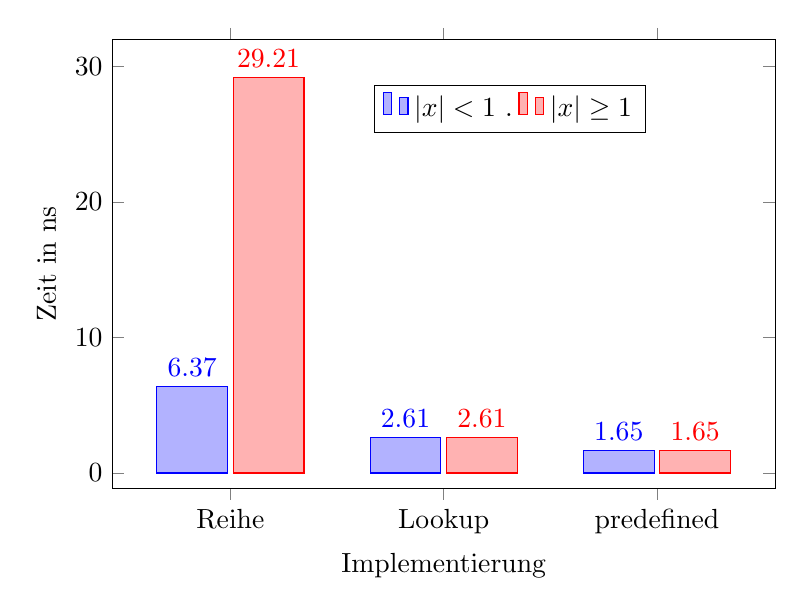
\begin{tikzpicture}
         \begin{axis}
             [
             ybar,
             width = 10 cm,
             height= \axisdefaultheight,
             bar width = 0.3 cm,
             enlarge x limits = {abs = 1.5 cm},
             symbolic x coords = {Reihe, Lookup,  predefined},
             xtick={Reihe, Lookup, predefined},
             ylabel={Zeit in ns},
             xlabel={Implementierung},
             legend style={at={(0.6, 0.9)},
               anchor=north,legend columns=-1},
             xtick=data,
             nodes near coords,
             nodes near coords align={vertical},
             bar width = 0.9cm,
             ]
             \addplot coordinates {(Reihe, 6.369) (Lookup, 2.613) (predefined, 1.648)};
             \addplot coordinates {(Reihe, 29.212) (Lookup, 2.613) (predefined, 1.648)};
             \legend{$|x|<1$  ., $|x|\geq 1$}
         \end{axis}
     \end{tikzpicture}
 
     \subsection{Bewertung, Einordnung und Erklärung der Ergebnisse}
     %Folgerungen
     Wie in der Abbildung zu sehen ist, ist die reine Reihen-Implementierung um ein Vielfaches (bis zu 12x) langsamer als die anderen
     beiden Vergleichsimplementierungen.
     Hier liegt auch die Stärke der Implementierung durch Lookup-Tabelle, die sogar mit der C-library mithalten kann.
     Der Grund für die Effizienz der Lookup-Tabelle ist, dass wir hier für jeden
     Input nur wenige billige arithmetische Ausdrücke sowohl für die Hashfunktion als auch zum linearen Interpolieren benötigen.
     Die Reihenentwicklung andererseits verwendet eine große Anzahl an Multiplikationen und Summen über eine Menge von Iterationen, was jedoch für eine Reihendarstellung mit Polynomen nicht zu vermeiden ist.
     \sout{Die Implementierung mit komplexen Instruktionen ist noch etwas schneller als unser Lookuptable, ist jedoch als Teil der
     C-library schwer zu unterbieten.}
 
     \section{Zusammenfassung und Ausblick}
     \subsection{Zusammenfassung}
     Zusammenfassend lässt sich feststellen, dass der Trade-off zwischen Performance, Genauigkeit und Speicherverbrauch für die beiden Implementierungen mit einem Tabellenlookup beziehungsweise einer Reihenentwicklung sehr unterschiedlich ist.
     Der Tabellenlookup ist zwar sehr schnell, benötigt allerdings auch immer mehr Speicherplatz, je genauere Werte man erhalten möchte.
     In unserer Implementierung, die insgesamt ca. 30000 Werte in einer Lookuptabelle speichert, hat die Berechnung einen maximalen relativen Fehler von bis zu etwa 0.01 Prozent.
 
     Die Reihenentwicklung auf der anderen Seite liefert zumindest für x-Werte, deren Betrag nicht nahe an Eins liegt, bereits mit wenigen Reihengliedern deutlich exaktere Werte.
     Allerdings werden beide Reihen für eine konstante Anzahl an Reihengliedern immer ungenauer, je näher sich x Eins annähert - um das exakte Ergebnis für Eins zu erhalten wäre eine unvertretbar hohe Anzahl an Reihengliedern erforderlich, die zu extremen Performanzeinbußen führen würden.
     Auch für die 20 Reihenglieder, für die wir uns entschieden haben, benötigt die Reihenentwicklung bis zu 12 mal so lange für die Berechnung, dafür benötigt sie auch deutlich weniger Speicherplatz.
 
 
     
     \subsection{Anwendung}
     Welches Programm verwendet werden sollte, hängt von den Rahmenbedingungen ab.
     In der Statistik kann der Areasinus Hyperbolicus zur Modellierung von Verteilungen verwendet werden, während er im Bereich des Ingenierwesens
     %TODO: Quelle für diese Aussage
     Anwendung in der Modellierung und Analyse von Systemen, beispielsweise in Steuerungs- und Regelungstechnik findet.~\cite{TODO}
     Für die Auswertung großer Messreihen zu diesem Zweck eignet sich die Lookuptabelle deutlich besser, da Messungen in der Regel sowieso einen kleinen Fehler aufweisen und die Lookuptabelle für viele Werte aufgrund der besseren Performanz schneller Ergebnisse liefert.
     Hat jedoch die exakte Genauigkeit der Ergebnisse ein höhere Priorität, so eignet sich die Reihenentwicklung mehr.
     Für x-Werte nahe an Eins müssen allerdings sehr viele Reihenglieder berechnet werden, da das Ergebnis andernfalls dennoch ungenau ausfällt.
 
     \subsection{Ausblick}
 
     In unserer Implementierung des $areasinus hyperbolicus$ haben wir uns auf eine reine Reihenentwicklung und eine einfache Lookup-Tabelle mit linearer Näherung beschränken müssen.
     Unter weniger strengen Rahmenbedingungen ließe sich die Implementierung allerdings sowohl in Bezug auf Laufzeit, als auch Genauigkeit noch signifikant optimieren. 
     
     Ein möglicher Ansatz ist die Verwendung von Splines in der Lookup-Tabelle: Statt der bisher linearen Näherung zwischen zwei Messpunkten in der Lookup-Tabelle, könnte man den $areasinus hyperbolicus$ in den Intervallen durch ein Polynom annähern.
     Hierzu werden in der Regel Polynome vom Grad drei verwendet. Das wäre eine Kombination der Genauigkeit und Speichereffizienz der Reihendarstellung und der Performanz der Lookup-Tabelle. 
     Dadurch verbessert sich die Genauigkeit, insbesondere für x-Werte die genau zwischen zwei Werten in der Lookup-Tabelle liegen deutlich, während sich die Laufzeit nur minimal erhöht.
     Dafür könnte allerdings der benötigte Speicherplatz steigen, da nun für jedes Intervall die Koeffizienten des Polynoms gespeichert werden müssten. Es könnte sich jedoch genauso herausstellen, dass durch die Polynominterpolation für eine hohe Genauigkeit eine geringere Dichte der Tabelleneinträge erforderlich ist, wodurch der Speicheraufwand wiederum sinken könnte.

     Ein weiterer Ansatz wäre, eine andere Art der Kombination aus Reihenentwicklung und Lookuptabelle zu verwenden: 
     Wie zuvor beobachtet liefert die Berechnung mit einer Reihenentwicklung für x-Werte, die nicht nahe an Eins liegen, besonders genaue Ergebnisse. Für |x|<0.125 brauchen wir beispielsweise nur 13 Reihenglieder, für |x|>8 brauchen wir 13 Reihenglieder der Restreihe, sowie bis zu 33 Reihenglieder der Taylorreihe für ein exaktes Ergebnis. In diesen Intervallen bietet es sich also durchaus an eine reine Reihenentwicklung zu verwenden. In dem Intervall 0.125<=|x|<=8 braucht man allerdings mehr Reihenglieder, wodurch es zu Performanzeinbußen kommt. Es wäre demnach sinnvoll in diesem Intervall eine Lookuptabelle zu verwenden. Da der Wertebereich nun deutlich kleiner ist, lassen sich bereits in kleinen Lookuptabellen, deutlich exaktere Werte speichern, wodurch der maximale relative Fehler minimal gehalten wird. Dieser Ansatz zielt besonders auf die Genauigkeit des Ergebnisses ab. Durch die Verwendung einer Lookuptabelle erhöht sich zudem die Performanz, da für die verbleibenden x-Werte weniger Reihenglieder berechnet werden müssen, um ein exaktes Ergebnis zu erhalten. 
     
     Welche Implementierung man nun wählt, hängt stark von der persönlichen Problemstellung ab. In den Fällen, in denen eine hohe Genauigkeit essentiell ist, wäre eine Variation mit Elementen einer Reihenentwicklung sinnvoll, solange man nicht eine große Menge Speicher zur Verfügung hat.
     Wenn die Implementatierung besonders schnell sein soll, sollte andererseits ein Lookup-Table benutzt werden.

     Anzumerken ist zudem, dass sich insbesondere die Reihenentwicklung durch die Verwendung von Assemblerinstruktionen noch signifikant auf Laufzeit optimieren lässt. 
 
 % TODO: Fuegen Sie Ihre Quellen der Datei Ausarbeitung.bib hinzu
 % Referenzieren Sie diese dann mit \cite{}.
 % Beispiel: CR2 ist ein Register der x86-Architektur~\cite{intel2017man}.
     \bibliographystyle{plain}
     \bibliography{Ausarbeitung}
 % Sämtliche in der Ausarbeitung verwendeten Quellen sind hier aufzuführen.
 % Es sollen nur zitierfähige Quellen verwendet werden. Wir empfehlen die Verwendung von BibTEX.
 
 \end{document}